\documentclass[10pt,letterpaper]{article}

\usepackage[top=0.6in, bottom=0.6in, left=0.68in, right=0.68in]{geometry}
\usepackage[utf8]{inputenc}
\usepackage[spanish,es-nodecimaldot]{babel}
\usepackage{amsmath,amssymb,amsfonts}
\usepackage{graphicx}
\usepackage{booktabs}
\usepackage{microtype}
\usepackage{xcolor}
\usepackage{cite}
\usepackage{enumitem}
\usepackage{subcaption}
\usepackage{url}
\usepackage{titlesec}

% Compactar espaciado de secciones
\titlespacing*{\section}{0pt}{7pt}{3pt}
\titlespacing*{\subsection}{0pt}{5pt}{2pt}
\setlist{nosep, leftmargin=1.2em}

% Espaciado de figuras
\setlength{\textfloatsep}{7pt plus 2pt minus 2pt}
\setlength{\floatsep}{6pt plus 2pt minus 2pt}
\setlength{\intextsep}{6pt plus 2pt minus 2pt}

\usepackage[colorlinks=true, linkcolor=blue!80!black, citecolor=blue!80!black, urlcolor=blue!80!black]{hyperref}

\title{\vspace{-1.3cm}\textbf{\Large Hoja de Trabajo \#2: Transformers y Mecanismos de Atención}\\
\normalsize CC3092 -- Deep Learning y Sistemas Inteligentes}
\author{\textbf{Javier España} (Carné: 23361) \quad | \quad Universidad del Valle de Guatemala\\
\normalsize Enlace al repositorio Git: \url{https://github.com/Javier-Espana/HT2-DL.git}}
\date{5 de octubre de 2026\vspace{-0.65cm}}

\begin{document}

\maketitle

\begin{abstract}
\small
Este informe analiza los fundamentos teóricos y experimentales de la arquitectura Transformer y los mecanismos de atención. Se examina la superación del cuello de botella de los modelos recurrentes (RNN seq2seq) mediante el mecanismo de Bahdanau, la analogía Query-Key-Value y las diferencias entre atención aditiva y multiplicativa. Se presenta la derivación matemática de la varianza en \textit{Scaled Dot-Product Attention} ($\mathrm{Var}(q\cdot k)=d_k$), justificando la necesidad de escalar por $\sqrt{d_k}$ para evitar el desvanecimiento de gradientes en la softmax. Mediante experimentación con \textsc{BERT} y \textsc{GPT-2}, se visualizan mapas de atención multifuncionales, se demuestra la resolución de correferencias en esquemas de Winograd, se cuantifica el fenómeno de sumideros de atención (\textit{attention sinks}) en arquitecturas autorregresivas y se evalúa la evolución de la entropía de atención a lo largo de las capas.
\end{abstract}

\vspace{-0.25cm}
\section{De las Redes Recurrentes a los Mecanismos de Atención}
\label{sec:rnn_atencion}

\textbf{Cuello de botella en seq2seq y solución de Bahdanau:}
En los modelos encoder-decoder recurrentes (RNN/LSTM/GRU), el encoder comprime la secuencia completa en un único vector de contexto estático $h_n \in \mathbb{R}^d$. Para oraciones largas, este vector representa un severo cuello de botella de capacidad informativa: los primeros tokens sufren desvanecimiento progresivo y pérdida irrecuperable de detalle fino debido a la acumulación sucesiva de no linealidades. Bahdanau et al.~\cite{bahdanau2014neural} resolvieron este problema permitiendo que el decoder consulte \textit{todos} los estados ocultos intermedios $\{h_1, \dots, h_n\}$. En cada paso $t$, se computa una distribución de atención $\alpha_{t,j}$ para formar un vector de contexto dinámico $c_t = \sum_{j=1}^n \alpha_{t,j} h_j$, manteniendo acceso directo a cualquier posición de la fuente sin compresión forzada.

\textbf{Atención aditiva vs. multiplicativa (Luong):}
Bahdanau et al.~\cite{bahdanau2014neural} introdujeron la atención aditiva usando una red multicapa: $e_{ij} = v_a^T \tanh(W_a s_{i-1} + U_a h_j)$. Por su parte, Luong et al.~\cite{luong2015effective} propusieron la atención multiplicativa o de producto punto: $e_{ij} = s_i^T W_a h_j$ (o $s_i^T h_j$). En hardware moderno (GPUs/TPUs), la atención multiplicativa es drásticamente más eficiente: se ejecuta como una única multiplicación matricial generalizada (GEMM), explotando al máximo los núcleos tensoriales con rutinas BLAS optimizadas en memoria contigua, mientras que la aditiva requiere asignar tensores intermedios y aplicar $\tanh$ elemento por elemento.

\textbf{Analogía Query ($Q$), Key ($K$) y Value ($V$):}
El mecanismo equivale a una búsqueda asociativa continua en un diccionario. En lugar de comparar una consulta con una clave binaria, la consulta $q$ evalúa su similitud con cada llave $k_i$. Tras normalizar las afinidades con softmax, se obtiene una combinación lineal ponderada de los valores: $\sum_i \alpha_i v_i$.
\begin{itemize}
    \item \textbf{Self-attention:} $Q, K, V$ nacen de la misma secuencia $X$, proyectada por matrices entrenables: $Q = X W^Q$, $K = X W^K$ y $V = X W^V$. Cada token contextualiza su representación atendiendo a todos los tokens del enunciado.
    \item \textbf{Cross-attention:} Las consultas $Q$ provienen del decodificador, mientras que las llaves $K$ y valores $V$ se extraen de la salida del codificador, guiando la generación condicionada por la fuente.
\end{itemize}

\textbf{Limitaciones superadas respecto a las RNNs:}
Al prescindir de la recurrencia, el Transformer elimina tres barreras: (1) \textit{Paralelismo masivo}: el procesamiento de la secuencia completa ocurre de forma simultánea en entrenamiento; (2) \textit{Longitud de camino $O(1)$}: cualquier par de tokens interactúa directamente en una capa de atención, frente a las $O(n)$ transiciones secuenciales de una RNN; (3) \textit{Estabilidad de gradiente}: se reduce el desvanecimiento de gradiente gracias a atajos residuales y atención directa.

\section{Arquitectura del Transformer}
\label{sec:arquitectura}

\textbf{Scaled Dot-Product Attention y derivación analítica de la varianza:}
La formulación es $\mathrm{Attention}(Q, K, V) = \mathrm{softmax}\left(\frac{Q K^T}{\sqrt{d_k}}\right) V$.
Sean $q, k \in \mathbb{R}^{d_k}$ dos vectores con componentes independientes e idénticamente distribuidos con media $\mathbb{E}[q_i]=\mathbb{E}[k_i]=0$ y varianza $\mathrm{Var}(q_i)=\mathrm{Var}(k_i)=1$. Su producto punto es $q \cdot k = \sum_{i=1}^{d_k} q_i k_i$. Para cada sumando:
\begin{equation}
    \mathbb{E}[q_i k_i] = \mathbb{E}[q_i]\mathbb{E}[k_i] = 0, \quad \mathrm{Var}(q_i k_i) = \mathbb{E}[(q_i k_i)^2] - (\mathbb{E}[q_i k_i])^2 = \mathrm{Var}(q_i)\mathrm{Var}(k_i) = 1.
\end{equation}
Por la propiedad de aditividad de la varianza para variables aleatorias independientes:
\begin{equation}
    \mathrm{Var}(q \cdot k) = \sum_{i=1}^{d_k} \mathrm{Var}(q_i k_i) = \sum_{i=1}^{d_k} 1 = d_k.
\end{equation}
La desviación estándar es $\sqrt{d_k}$. Si se divide entre $\sqrt{d_k}$, la varianza se normaliza a la unidad:
\begin{equation}
    \mathrm{Var}\left(\frac{q \cdot k}{\sqrt{d_k}}\right) = \frac{1}{d_k}\mathrm{Var}(q \cdot k) = \frac{d_k}{d_k} = 1.
\end{equation}
\textit{Efecto en la softmax sin escalamiento:} Para dimensiones habituales ($d_k=64$ o $128$), el producto punto alcanza magnitudes de orden $\sqrt{d_k} \approx 8 - 11$. Al alimentar logits tan dispares a la función softmax ($S_i = e^{z_i}/\sum_j e^{z_j}$), la distribución se polariza hacia un vector casi \textit{one-hot}. Dado que la derivada es $\frac{\partial S_i}{\partial z_j} = S_i(\delta_{ij} - S_j)$, cuando $S_i \to 1$ o $S_i \to 0$ el gradiente colapsa exponencialmente hacia cero, deteniendo el aprendizaje de los pesos por desvanecimiento del gradiente.

\textbf{Multi-Head Attention (MHA):}
MHA proyecta las entradas a $h$ subespacios independientes de menor dimensión $d_k = d_{\text{model}}/h$:
\begin{equation}
    \mathrm{MHA}(Q, K, V) = \mathrm{Concat}(\mathrm{head}_1, \dots, \mathrm{head}_h) W^O, \quad \mathrm{head}_i = \mathrm{Attention}(Q W_i^Q, K W_i^K, V W_i^V).
\end{equation}
Esto permite al modelo atender simultáneamente a múltiples aspectos complementarios (sintaxis local, correferencia pronominal, dependencias semánticas de largo alcance). El número de parámetros \textbf{no cambia}: las $h$ cabezas con matrices de tamaño $d_{\text{model}} \times (d_{\text{model}}/h)$ suman $h \cdot \frac{d_{\text{model}}^2}{h} = d_{\text{model}}^2$ por proyección, idéntico a una sola proyección de dimensión completa.

\textbf{Codificación Posicional:}
La auto-atención pura es una operación equivariante a permutaciones: permutar el orden de los tokens de entrada permuta exactamente las salidas sin registrar alteración de significado. Para codificar el orden secuencial se inyectan embeddings de posición:
\begin{itemize}
    \item \textit{Sinusoidal fija~\cite{vaswani2017attention}:} Funciones seno y coseno de frecuencias geométricas ($PE_{(pos, 2i)} = \sin(pos/10000^{2i/d})$). Permiten modelar desplazamientos relativos mediante combinaciones lineales y extrapolar a longitudes mayores.
    \item \textit{Embeddings aprendidos (BERT, GPT-2):} Matrices entrenables $L_{\max} \times d_{\text{model}}$. Son altamente expresivas pero incapaces de generalizar más allá de su longitud prefijada.
    \item \textit{RoPE (Rotary Position Embedding)~\cite{su2024roformer}:} Rota los vectores $Q$ y $K$ en el plano complejo con ángulos proporcionales a su posición: el producto $(\tilde{q}_m)^T \tilde{k}_n$ codifica naturalmente la distancia relativa $(n-m)$, conservando la norma euclidiana y facilitando extrapolación de contexto.
\end{itemize}

\textbf{Bloque Transformer: Conexiones residuales, LayerNorm y MLP:}
Cada bloque integra MHA y una red feed-forward bi-lineal por posición ($\mathrm{FFN}(x) = \max(0, x W_1 + b_1) W_2 + b_2$) con dimensión interna $4 d_{\text{model}}$. En \textit{Post-LN}~\cite{vaswani2017attention}, la normalización se sitúa tras la suma residual ($x_{l+1} = \mathrm{LN}(x_l + \mathrm{Sublayer}(x_l))$), lo que introduce gradientes inestables en las primeras capas y demanda fases estrictas de calentamiento (\textit{warmup}). En cambio, \textit{Pre-LN} aplica la normalización a la entrada de cada subcapa ($x_{l+1} = x_l + \mathrm{Sublayer}(\mathrm{LN}(x_l))$), preservando un canal residual sin distorsión que garantiza convergencia robusta sin warmup hipercalibrado.

\textbf{Complejidad y alternativas eficientes:}
El producto $QK^T$ requiere $O(n^2 d)$ operaciones y $O(n^2)$ en memoria de activación por cabeza. Principales propuestas de mitigación:
\begin{itemize}
    \item \textit{FlashAttention~\cite{dao2022flashattention}:} Calcula softmax en bloques sobre memoria SRAM rápida sin escribir la matriz $n \times n$ en memoria global (HBM). Es exacta (sin aproximación), pero requiere kernels específicos de bajo nivel.
    \item \textit{Atención por ventanas / Sparse (Longformer):} Limita la atención a un entorno local de tamaño $w \ll n$, con costo $O(n \cdot w)$, sacrificando interacción global directa en una sola capa.
    \item \textit{Atención lineal (Linformer, Performer):} Aplica descomposición de kernel para operar $Q(K^T V)$ en costo $O(n d^2)$, sacrificando la precisión de la distribución softmax pura.
\end{itemize}

\begin{figure}[t]
    \centering
    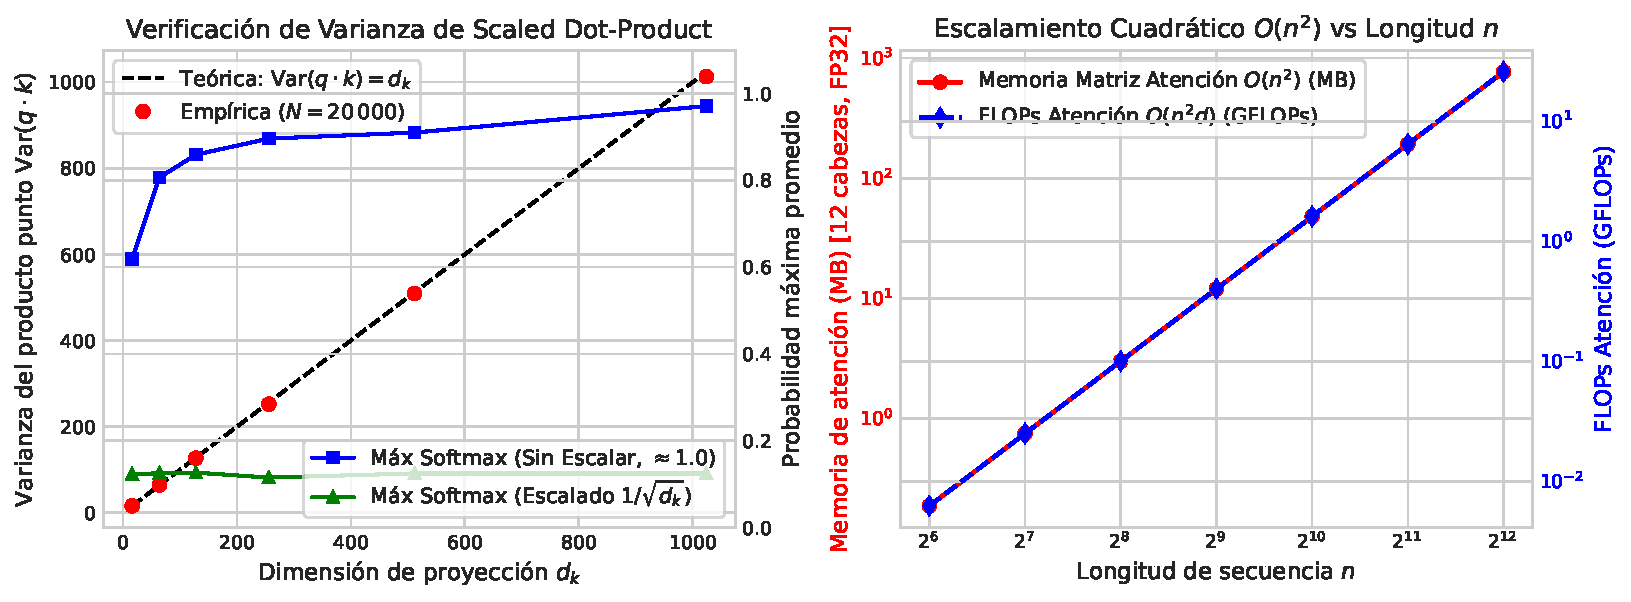
\includegraphics[width=0.82\linewidth]{figures/fig_scaling_complexity.pdf}
    \vspace{-0.2cm}
    \caption{\textbf{Izquierda:} Verificación empírica de $\mathrm{Var}(q \cdot k) = d_k$ y saturación del valor máximo de la Softmax cuando se prescinde de $\sqrt{d_k}$. \textbf{Derecha:} Escalamiento cuadrático $O(n^2)$ de memoria y FLOPs vs. longitud de secuencia $n$.}
    \label{fig:scaling}
    \vspace{-0.25cm}
\end{figure}

\section{Atención en PyTorch y Hugging Face}
\label{sec:pytorch_hf}
\begin{itemize}
    \item \texttt{F.scaled\_dot\_product\_attention}: Función optimizada en PyTorch 2.x con despacho automático a FlashAttention o kernels nativos. Recibe \texttt{query}, \texttt{key}, \texttt{value}, y argumentos clave: \texttt{attn\_mask} (máscara aditiva o booleana), \texttt{dropout\_p}, \texttt{is\_causal} (máscara causal rápida) y \texttt{scale} (factor de escala alternativo).
    \item \texttt{nn.MultiheadAttention}: Módulo de atención multi-cabeza (\texttt{embed\_dim}, \texttt{num\_heads}, \texttt{batch\_first}, \texttt{kdim}, \texttt{vdim}). Su método \texttt{forward} admite \texttt{key\_padding\_mask} para omitir relleno (\textit{padding}), \texttt{attn\_mask}, \texttt{need\_weights} y \texttt{average\_attn\_weights} (promedio o discriminación por cabeza).
    \item \texttt{nn.TransformerEncoderLayer}: Capa completa con \texttt{d\_model}, \texttt{nhead}, \texttt{dim\_feedforward}, \texttt{dropout} y \texttt{norm\_first} (Pre-LN vs Post-LN). Con \texttt{generate\_square\_subsequent\_mask(sz)} crea la máscara triangular causal rellena de $-\infty$.
    \item \textbf{Atención en Hugging Face:} Al invocar un modelo con \texttt{output\_attentions=True}, la salida incluye \texttt{attentions}: tupla de $L$ tensores (uno por capa) de dimensiones \texttt{[batch\_size, num\_heads, seq\_len, seq\_len]}.
\end{itemize}

\section{Ejercicios Prácticos y Verificaciones Empíricas}
\label{sec:practica}

\begin{figure}[t]
    \centering
    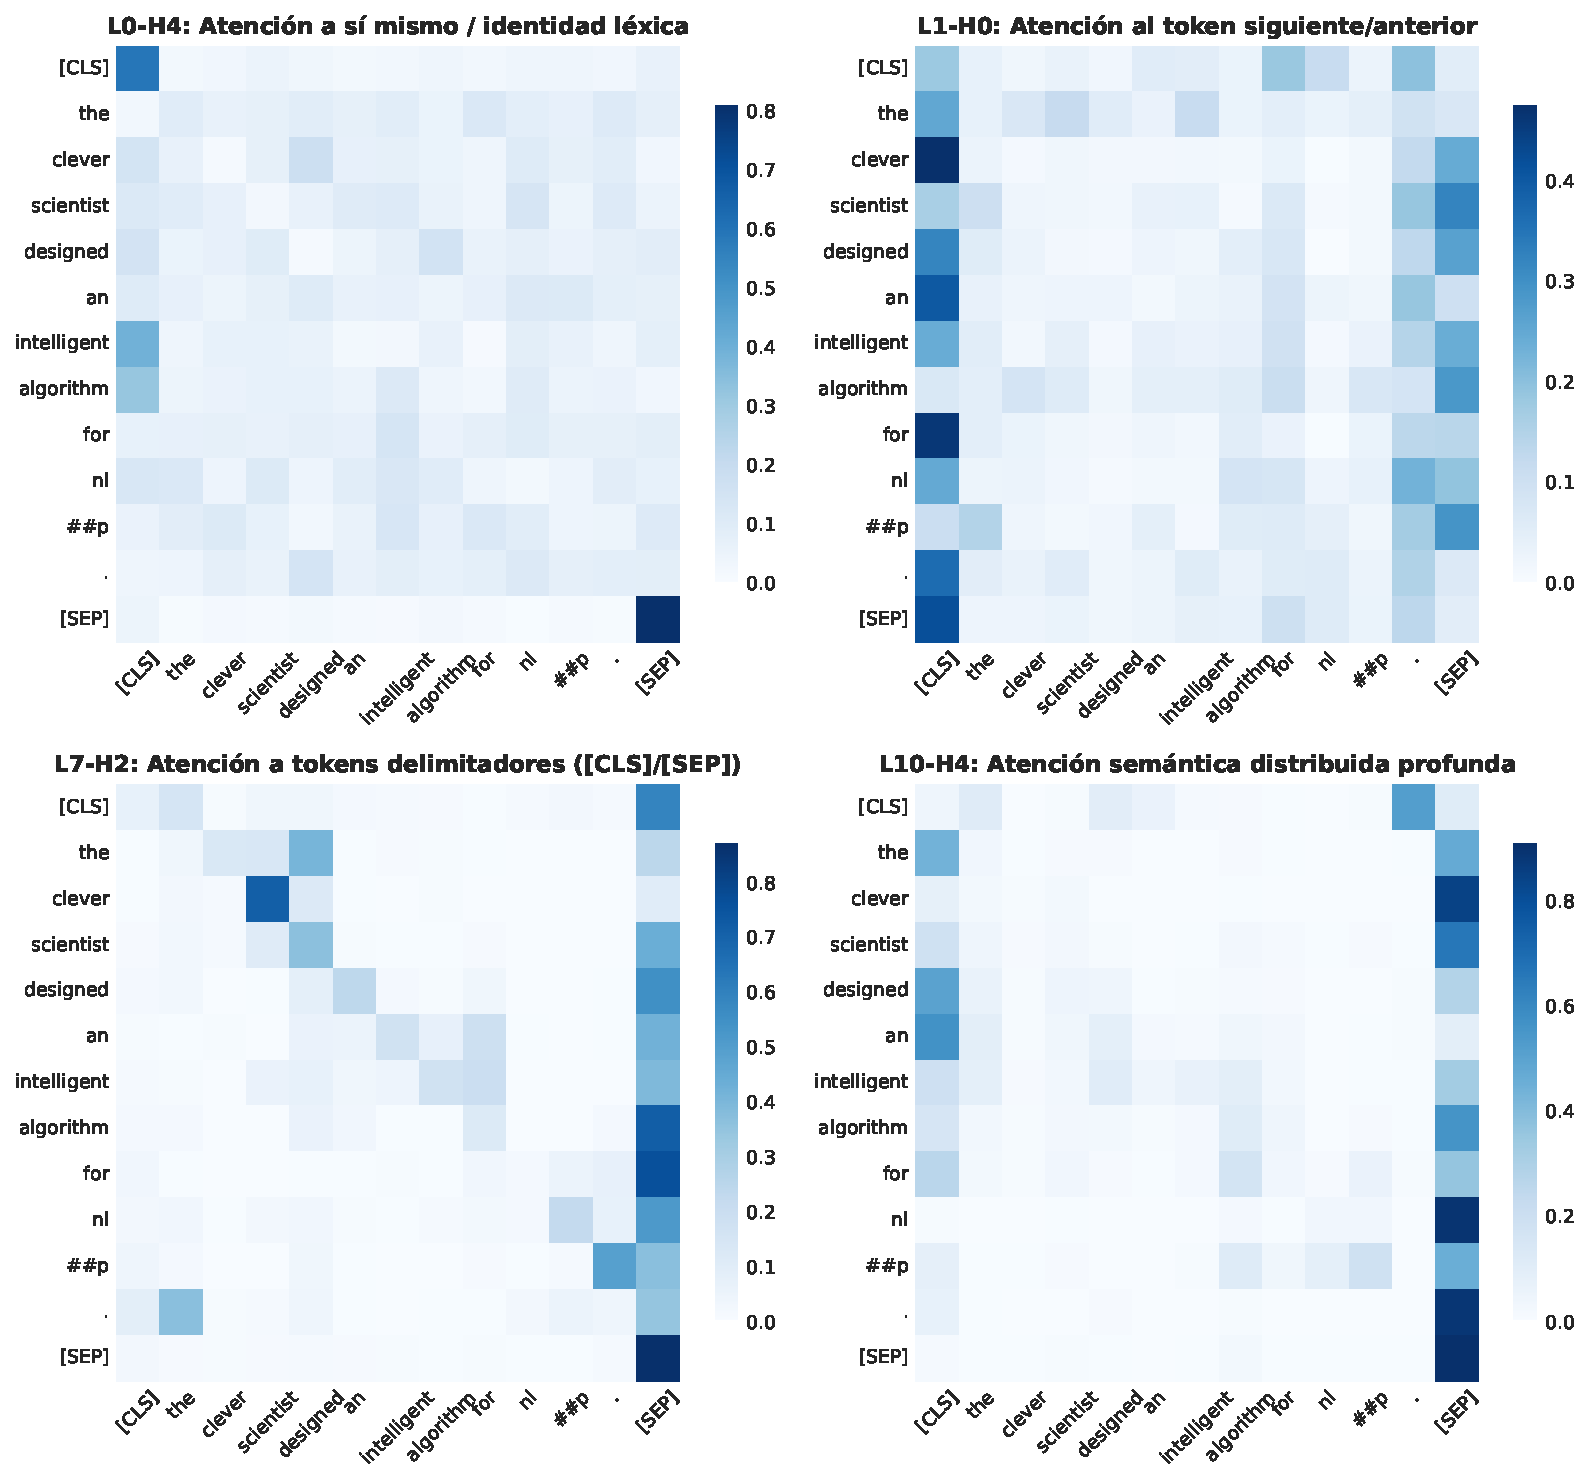
\includegraphics[width=0.68\linewidth]{figures/fig_bert_heatmaps.pdf}
    \vspace{-0.2cm}
    \caption{Mapas de calor en \textsc{BERT} mostrando cuatro patrones: identidad léxica (L0-H4), atención a token adyacente (L1-H0), concentración en delimitadores especiales \texttt{[CLS]} y \texttt{[SEP]} (L7-H2) y dispersión semántica contextual (L10-H4).}
    \label{fig:bert_heatmaps}
    \vspace{-0.25cm}
\end{figure}

\textbf{Verificación numérica y ejercicio de escalamiento:}
Generamos $20\,000$ pares de vectores gaussianos $q, k \sim \mathcal{N}(0, I)$ para dimensiones $d_k \in \{16, 64, 128, 256, 512, 1024\}$. Como ilustra la Figura~\ref{fig:scaling} (izquierda), las varianzas observadas fueron $[16.16, 64.67, 127.08, 252.39, 509.24, 1012.72]$, validando empíricamente que $\mathrm{Var}(q \cdot k) = d_k$. Sin la división entre $\sqrt{d_k}$, la probabilidad máxima de la softmax satura rápidamente hacia $0.971$, eliminando gradientes, mientras que con el factor escala se conserva equilibrada cerca de $0.125$. Asimismo, la implementación manual desarrollada en el notebook produjo salidas numéricas idénticas a PyTorch ($<10^{-6}$). En la Figura~\ref{fig:scaling} (derecha) se constata el crecimiento de memoria (768 MB por capa a 4096 tokens) y FLOPs característicos de $O(n^2)$.

\textbf{Mapas de calor en BERT:}
En la Figura~\ref{fig:bert_heatmaps} evaluamos la oración \textit{``The clever scientist designed an intelligent algorithm for NLP.''} en \textsc{BERT}, identificando cuatro patrones canónicos:
\begin{enumerate}
    \item \textit{Atención a la propia palabra (L0-H4):} Fuerte concentración diagonal que preserva los embeddings iniciales.
    \item \textit{Tokens adyacentes (L1-H0):} Banda subdiagonal orientada al token contiguo (\textit{clever} $\to$ \textit{scientist}).
    \item \textit{Delimitadores especiales (L7-H2):} Absorción en \texttt{[CLS]} y \texttt{[SEP]} actuando como comodines neutros.
    \item \textit{Semántica contextual profunda (L10-H4):} Conexiones cruzadas y no locales entre términos afines.
\end{enumerate}

\begin{figure}[t]
    \centering
    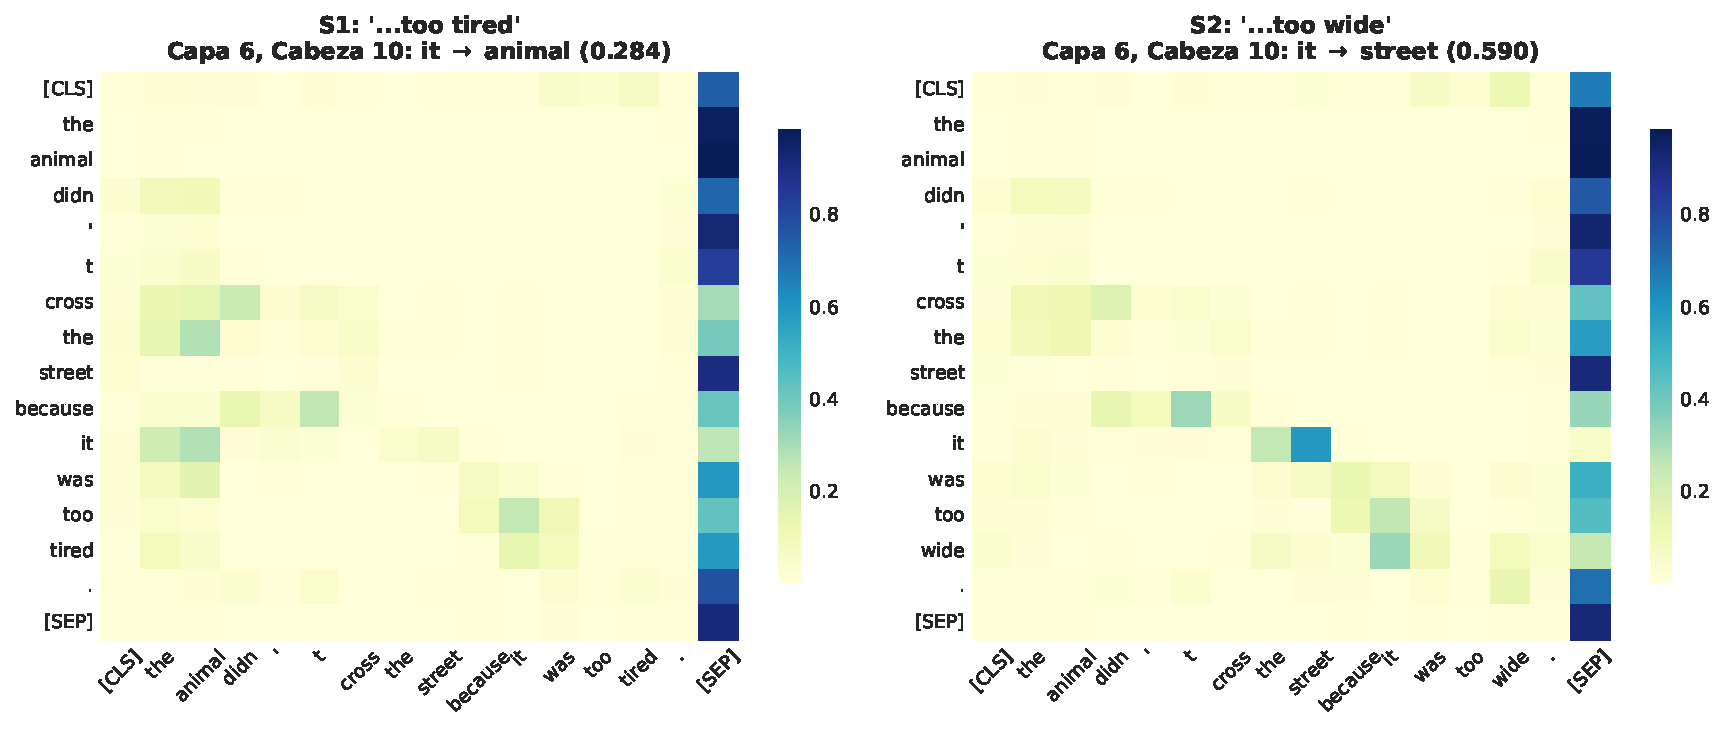
\includegraphics[width=0.78\linewidth]{figures/fig_winograd_resolution.pdf}
    \vspace{-0.2cm}
    \caption{Resolución de correferencia en esquema Winograd con \textsc{BERT} (Capa 6, Cabeza 10). En $S_1$ (\textit{too tired}), \textit{it} atiende fuertemente a \textit{animal} ($0.284$). En $S_2$ (\textit{too wide}), la atención de \textit{it} cambia radicalmente hacia \textit{street} ($0.590$).}
    \label{fig:winograd}
    \vspace{-0.25cm}
\end{figure}

\textbf{Resolución de correferencias (Esquema de Winograd):}
Analizamos el par:
\begin{itemize}
    \item $S_1$: \textit{``The animal didn't cross the street because it was too tired.''}
    \item $S_2$: \textit{``The animal didn't cross the street because it was too wide.''}
\end{itemize}
Exploramos las 144 cabezas de \textsc{BERT} buscando maximizar el contraste de atención de \textit{``it''} hacia \textit{``animal''} en $S_1$ y hacia \textit{``street''} en $S_2$. La \textbf{Capa 6, Cabeza 10} arrojó la máxima desambiguación ($\Delta = 0.7954$): en $S_1$ asigna $0.2843$ a \textit{animal} y solo $0.0671$ a \textit{street}; en $S_2$ asigna $0.5902$ a \textit{street} y $0.0119$ a \textit{animal} (Figura~\ref{fig:winograd}), comprobando que el modelo resuelve correferencias sintáctico-semánticas en capas intermedias.

\begin{figure}[t]
    \centering
    \begin{subfigure}[b]{0.56\linewidth}
        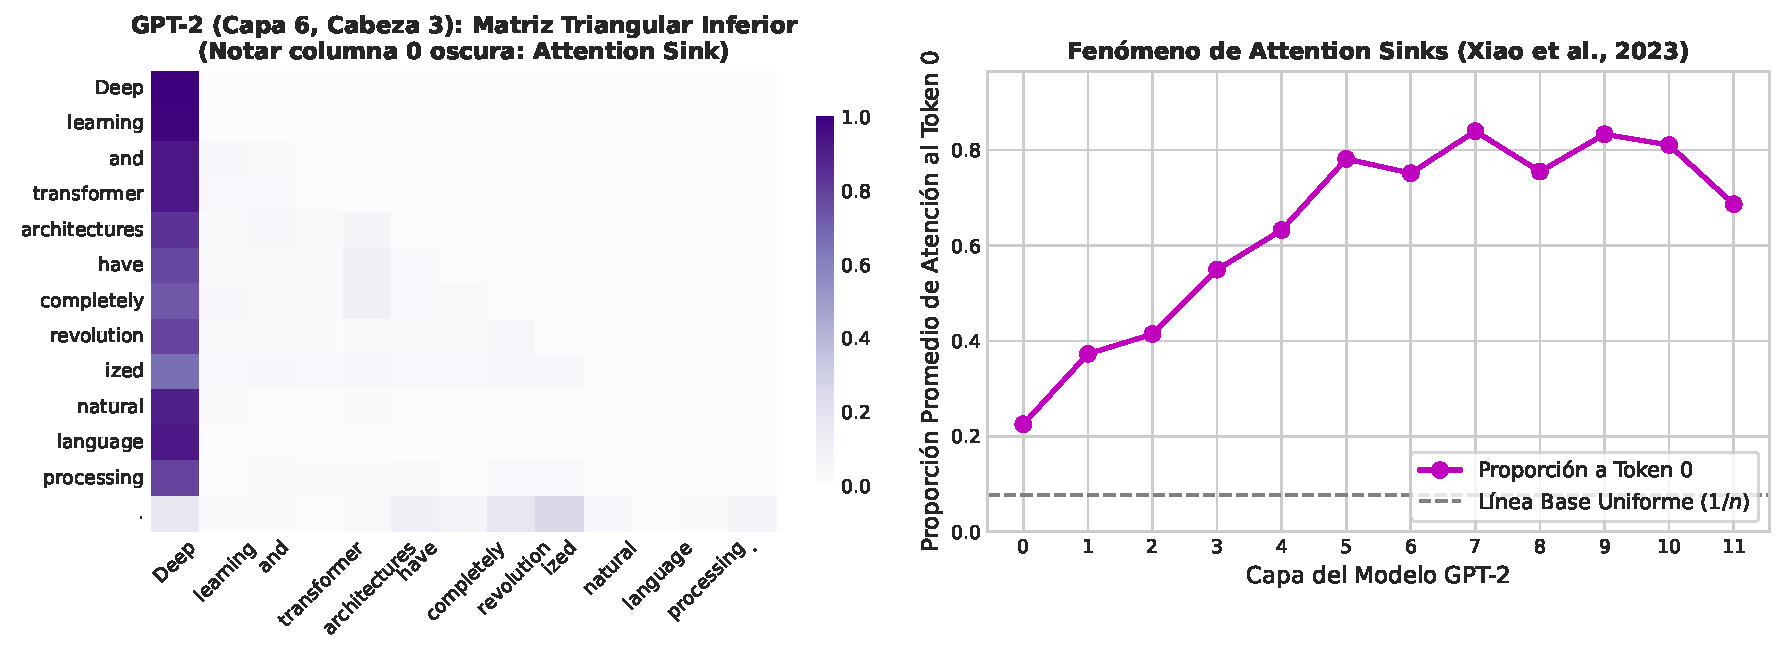
\includegraphics[width=\linewidth]{figures/fig_gpt2_causal_sinks.pdf}
        \caption{Máscara causal y proporción a Token 0 en \textsc{GPT-2}.}
        \label{fig:sinks}
    \end{subfigure}
    \hfill
    \begin{subfigure}[b]{0.41\linewidth}
        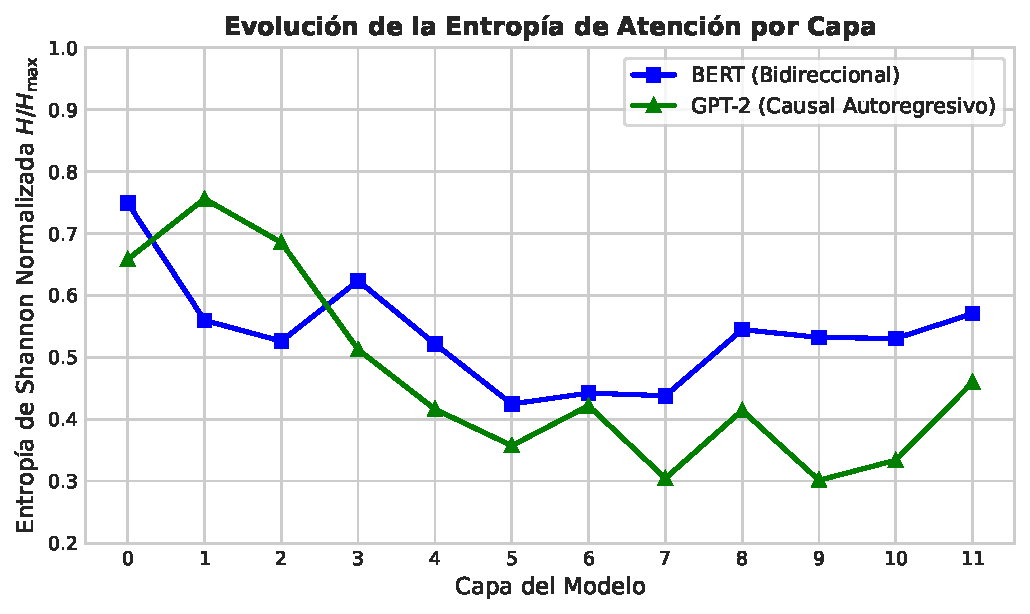
\includegraphics[width=\linewidth]{figures/fig_attention_entropy.pdf}
        \caption{Entropía normalizada por capa.}
        \label{fig:entropy}
    \end{subfigure}
    \vspace{-0.2cm}
    \caption{\textbf{(a)} Causalidad triangular inferior y \textit{attention sinks} en \textsc{GPT-2}. \textbf{(b)} Dinámica de entropía: las capas profundas se tornan más concentradas (menor entropía).}
    \label{fig:gpt2_and_entropy}
    \vspace{-0.25cm}
\end{figure}

\textbf{Atención causal y Attention Sinks en GPT-2:}
Verificamos computacionalmente que la matriz de atención de \textsc{GPT-2} es estrictamente triangular inferior (valores sobre la diagonal idénticamente nulos). Al estudiar la distribución de pesos, confirmamos de forma rotunda el fenómeno de \textbf{Attention Sinks}~\cite{xiao2023efficient}: el \texttt{token 0} recibe en promedio el $22.5\%$ de atención en la capa 0, pero a partir de la capa 4 absorbe entre el \textbf{$75\%$ y el $84\%$} de la atención de los tokens posteriores (Figura~\ref{fig:sinks}). Esto ocurre porque la softmax impone que las sumas de fila sean 1; al no requerir atención sustantiva en ciertos pasos, el modelo vierte el exceso numérico en el primer token disponible.

\textbf{Entropía de atención por capa (BERT vs. GPT-2):}
Calculamos la entropía de Shannon normalizada $H/H_{\max}$ (Figura~\ref{fig:entropy}). En ambos modelos, las capas iniciales exhiben entropía elevada ($0.75-0.76$), correspondiente a distribuciones dispersas. En capas intermedias y profundas, la entropía decae marcadamente ($0.42$ en BERT y $0.30$ en GPT-2), reflejando una focalización especializada en dependencias concretas.

\section{Discusión y Análisis Crítico}
\label{sec:discusion}

\textbf{1. Ventajas de escalamiento frente a RNNs:}
El entrenamiento de RNNs estaba encadenado al paso temporal $h_t = f(h_{t-1}, x_t)$, imposibilitando paralelizar la secuencia en GPUs. Además, el camino informacional $O(n)$ degradaba los gradientes. La auto-atención sustituyó la recurrencia por álgebra lineal paralelizable masiva en un paso constante $O(1)$. Pese al costo cuadrático, la regularidad del flujo computacional permitió expandir los modelos hacia las leyes de escala de Chinchilla/Kaplan.

\textbf{2. Especialización y redundancia de cabezas:}
Aunque identificamos cabezas altamente especializadas (ej. correferencia en L6-H10), trabajos canónicos de poda (\textit{pruning})~\cite{voita2019analyzing} demuestran que una porción notable de cabezas puede descartarse durante la inferencia sin merma de desempeño; el grueso del trabajo crítico recae sobre un núcleo reducido de cabezas.

\textbf{3. ¿Los pesos de atención son explicación causal?}
Jain y Wallace~\cite{jain2019attention} mostraron que distribuciones de atención completamente diferentes pueden generar idéntica predicción, arguyendo que ``atención no es explicación''. Wiegreffe y Pinter~\cite{wiegreffe2019attention} precisaron que la atención refleja el flujo intermedio de información, pero debido a la no linealidad de las FFN subsecuentes, los pesos de atención describen correlaciones de representación y no causalidad estricta.

\textbf{4. Cuándo preferir una RNN o CNN sobre un Transformer:}
Las RNNs (y arquitecturas afines como Mamba o RWKV) siguen siendo preferibles en dispositivos con memoria RAM ultrarreducida (Edge/TinyML) gracias a su inferencia con memoria constante $O(1)$, evitando el costo del KV cache. Por su parte, las CNNs ofrecen un sesgo inductivo traslacional insustituible para visión o audio crudo de bajo costo paramétrico.

\textbf{5. Procesamiento de secuencias de 100,000 tokens:}
Una secuencia de $10^5$ tokens colapsa la memoria convencional (requiriendo cientos de gigabytes solo para matrices de atención). Las soluciones estándar incluyen: FlashAttention-2 acoplado a RingAttention (paralelismo entre GPUs), ventanas de atención deslizante con \textit{attention sinks} fijos (StreamingLLM), modelos de estado en el espacio (Mamba) con memoria $O(1)$ en generación, y arquitecturas de recuperación aumentada (RAG).

\section{Conclusiones}
\label{sec:conclusiones}

El mecanismo de atención redefinió el procesamiento de secuencias eliminando el cuello de botella recurrente. Verificamos que el factor $1/\sqrt{d_k}$ estabiliza la varianza unitaria de los logits e impide el colapso de gradientes en la softmax. Los análisis empíricos confirman la especialización de cabezas en BERT y la naturaleza de sumidero numérico del token inicial en GPT-2. La combinación de estos principios sustenta los avances contemporáneos del Deep Learning.

\vspace{0.15cm}
\noindent\textbf{Repositorio Git del proyecto:} \url{https://github.com/Javier-Espana/HT2-DL.git}

\vspace{-0.1cm}
\small
\bibliographystyle{IEEEtran}
\bibliography{referencias}

\end{document}
